% ============================================================
%  Modul 2 — Instalasi Ubuntu di VirtualBox
% ============================================================

\chapter{Instalasi Ubuntu di VirtualBox}
\label{chap:modul-02}

% --- 1. Tujuan dan Output Praktikum ---
\section{Tujuan dan Output Praktikum}

\subsection{Tujuan Praktikum}
Setelah menyelesaikan praktikum ini, mahasiswa diharapkan mampu:
\begin{enumerate}
    \item Menjelaskan langkah-langkah instalasi sistem operasi Ubuntu pada lingkungan VirtualBox.
    \item Mengonfigurasi mesin virtual sesuai dengan kebutuhan sistem (alokasi RAM, storage, dan CPU).
    \item Melakukan proses instalasi Ubuntu hingga sistem dapat dijalankan dengan baik sebagai Guest Operating System.
\end{enumerate}

\subsection{Output Praktikum}
Pada akhir praktikum ini, mahasiswa diharapkan menghasilkan:
\begin{itemize}
    \item Mesin virtual Ubuntu yang berhasil terinstal dan dapat dijalankan pada VirtualBox.
    \item Dokumentasi proses instalasi (screenshot tahapan penting instalasi).
    \item Laporan praktikum yang memuat konfigurasi mesin virtual serta hasil verifikasi sistem.
\end{itemize}


% --- 2. Dasar Teori ---
\newpage
\section{Dasar Teori}

\subsection{Konsep Virtualisasi dan Peran VirtualBox}
Virtualisasi adalah teknik untuk menjalankan sistem komputer virtual di atas komputer fisik yang sama. Pada praktikum ini, sistem operasi utama pada laptop atau PC Anda berperan sebagai \textit{host operating system}, sedangkan Ubuntu yang akan dipasang di dalam VirtualBox berperan sebagai \textit{guest operating system}. VirtualBox sendiri bertindak sebagai \textit{hypervisor type-2}, yaitu perangkat lunak yang meminjam sebagian sumber daya \textit{host} (CPU, RAM, penyimpanan, dan perangkat I/O) lalu menyajikannya sebagai mesin virtual mandiri bagi \textit{guest}.

Pendekatan ini penting dalam praktikum sistem operasi karena memberi lingkungan yang aman dan terisolasi. Kesalahan konfigurasi, eksperimen perintah, atau kegagalan \textit{boot} di dalam Ubuntu tidak langsung merusak sistem utama pengguna. Selain itu, seluruh mahasiswa dapat bekerja dengan lingkungan Linux yang relatif seragam meskipun komputer \textit{host}-nya berbeda-beda.

File \texttt{ISO} Ubuntu yang digunakan pada modul ini adalah citra media instalasi. Secara konseptual, berkas ini setara dengan keping DVD instalasi, hanya saja berbentuk file. Saat file ISO dipasangkan ke VM, firmware virtual akan melakukan \textit{boot} dari ISO tersebut dan memulai program instalasi Ubuntu.

\subsection{Komponen Konfigurasi Mesin Virtual}
Sebelum instalasi dimulai, VirtualBox meminta beberapa parameter konfigurasi. Masing-masing parameter memiliki fungsi teknis yang perlu dipahami agar pengaturan VM tidak dilakukan sekadar mengikuti klik antarmuka.

\begin{itemize}
    \item \textbf{Name}: penanda administrasi VM pada VirtualBox. Nama ini memudahkan identifikasi, tetapi tidak memengaruhi kinerja sistem.
    \item \textbf{ISO Image}: sumber media \textit{boot} awal yang berisi installer Ubuntu.
    \item \textbf{Username}, \textbf{Password}, dan \textbf{Hostname}: identitas akun awal dan nama mesin yang akan dipakai setelah instalasi selesai.
    \item \textbf{Base Memory (RAM)}: jumlah memori fisik \textit{host} yang dipinjam sementara oleh VM saat dijalankan. Jika terlalu kecil, installer dan sistem Ubuntu akan terasa lambat; jika terlalu besar, sistem \textit{host} dapat ikut kekurangan memori.
    \item \textbf{Processor}: jumlah inti CPU virtual yang dialokasikan. Menambah inti dapat mempercepat pekerjaan tertentu, tetapi alokasi berlebihan juga dapat membuat \textit{host} tidak responsif.
    \item \textbf{Virtual Hard Disk}: ruang penyimpanan virtual tempat Ubuntu, aplikasi, dan data \textit{guest} disimpan. Disk ini biasanya berupa file besar pada mesin \textit{host}.
\end{itemize}

Prinsip umumnya adalah membagi sumber daya secara seimbang. VM harus mendapat sumber daya yang cukup untuk berjalan lancar, tetapi sistem \textit{host} tetap harus menyisakan kapasitas agar VirtualBox dan aplikasi pendukung lain tetap stabil.

\subsection{Tahapan Umum Instalasi Ubuntu}
Secara umum, instalasi Ubuntu di VM berlangsung melalui empat tahap. Pertama, VM melakukan \textit{boot} dari file ISO dan menjalankan program installer. Kedua, installer menyalin berkas sistem dasar Ubuntu ke \textit{virtual hard disk}. Ketiga, installer membuat akun pengguna, nama komputer, dan konfigurasi awal lain. Keempat, sistem melakukan \textit{restart} dan \textit{boot} ulang dari disk virtual yang baru saja diisi, bukan lagi dari file ISO.

Memahami alur ini membantu mahasiswa membaca gejala saat instalasi berlangsung. Misalnya, jika VM gagal \textit{boot} dari awal, masalah biasanya berada pada pemilihan ISO atau urutan \textit{boot}. Jika proses sangat lambat, penyebab umumnya adalah alokasi RAM/CPU yang terlalu kecil. Jika setelah \textit{restart} sistem kembali ke installer, kemungkinan media \textit{boot} masih mengarah ke ISO, bukan ke disk virtual hasil instalasi.

Tabel \ref{tab:m02-dasar-teori} merangkum komponen inti yang perlu dipahami sebelum praktik instalasi.

\begin{table}[h]
\caption{Tabel Ringkasan Dasar Teori Modul 2}
\label{tab:m02-dasar-teori}
\centering
\begin{tabulary}{\textwidth}{|L|L|}
\hline
\textbf{Konsep} & \textbf{Penjelasan Singkat} \\ \hline
Host OS & Sistem operasi utama pada komputer fisik yang menjalankan VirtualBox. \\ \hline
Guest OS & Sistem operasi tamu (Ubuntu) yang dipasang dan dijalankan di dalam mesin virtual. \\ \hline
Hypervisor Type-2 & Perangkat lunak virtualisasi yang berjalan di atas \textit{host OS} untuk membuat dan mengelola VM. \\ \hline
ISO Image & Berkas citra instalasi yang digunakan VM sebagai media \textit{boot} awal. \\ \hline
Base Memory / Processor & Parameter alokasi sumber daya yang menentukan performa VM dan beban pada \textit{host}. \\ \hline
Virtual Hard Disk & Berkas penyimpanan virtual yang menjadi media instalasi dan data Ubuntu di dalam VM. \\ \hline
\end{tabulary}
\end{table}


% --- 3. Alat dan Bahan ---
\section{Alat dan Bahan}
\label{sec:alat-bahan}

\subsection{Perangkat Keras}
Untuk dapat menjalankan instalasi Ubuntu pada lingkungan virtual, diperlukan perangkat keras dengan spesifikasi minimum sebagai berikut:
\begin{itemize}
    \item Laptop atau PC dengan prosesor minimal dual-core.
    \item RAM minimal 4 GB (disarankan 8 GB untuk kinerja optimal).
    \item Ruang penyimpanan kosong minimal 25 GB.

\end{itemize}
Spesifikasi yang lebih tinggi akan meningkatkan performa mesin virtual selama proses instalasi dan penggunaan sistem.

\subsection{Perangkat Lunak}
Perangkat lunak yang diperlukan dalam praktikum ini meliputi:
\begin{itemize}
    \item Sistem Operasi utama (Windows, macOS, atau Linux) sebagai Host OS.
    \item Oracle VM VirtualBox 
    \item File ISO Ubuntu .
\end{itemize}
Pastikan VM VirtualBox dan file ISO Ubuntu telah diunduh sebelum praktikum dimuli untuk menghindari keterlambatan proses instalasi.

% --- 4. Langkah-Langkah Praktikum ---
\newpage
\section{Langkah-Langkah Praktikum}

\begin{enumerate}
    \item \textbf{Instalasi VirtualBox}

    Langkah pertama yang harus dilakukan adalah menginstal software virtualisasi, yaitu Oracle VM VirtualBox.

    Unduh VirtualBox melalui tautan resmi berikut:

    \url{https://www.virtualbox.org/wiki/Downloads}

    \item \textbf{Mengunduh File ISO Ubuntu Desktop}

    Setelah VirtualBox berhasil diinstal, langkah berikutnya adalah menyiapkan sistem operasi yang akan dijalankan di dalam Virtual Machine, yaitu Ubuntu Desktop.

    Unduh file ISO Ubuntu Desktop melalui tautan resmi berikut:

    \url{https://ubuntu.com/download/desktop}

    \item \textbf{Setup Virtual Machine}

    Setelah VirtualBox terinstal dan file ISO Ubuntu sudah diunduh, langkah selanjutnya adalah melakukan setup Virtual Machine di VirtualBox.

    \begin{enumerate}
        \item Buka aplikasi Oracle VM VirtualBox, kemudian klik tombol \textbf{New}.

        \begin{figure}[H]
            \centering
            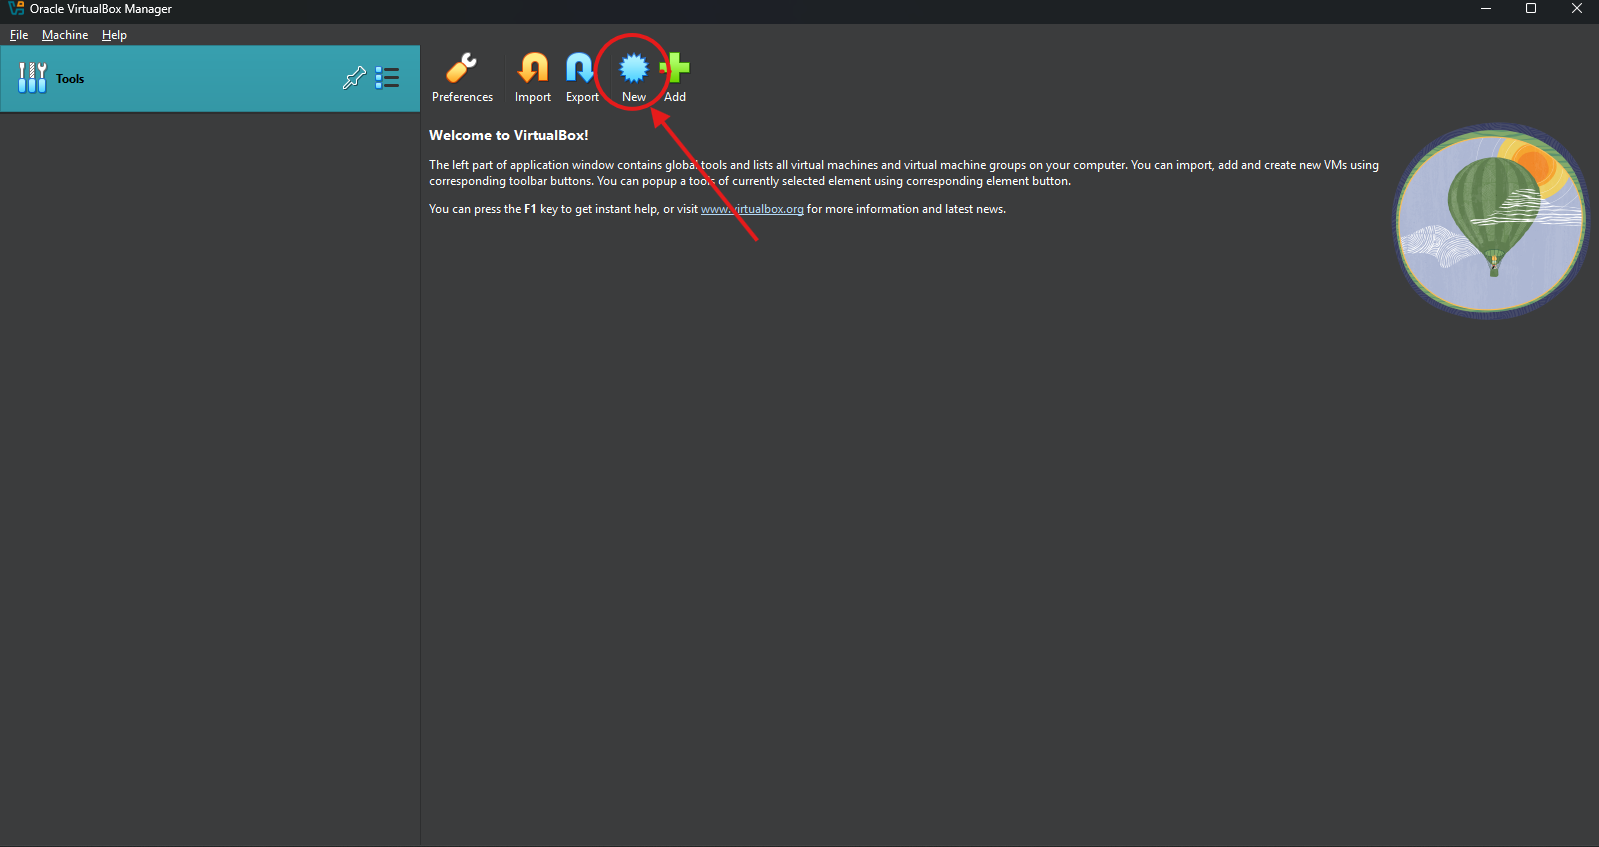
\includegraphics[width=0.75\textwidth]{Figure/02/gambar1.png}
            \caption{Tampilan Oracle VM VirtualBox saat memilih tombol \textbf{New}.}
            \label{fig:virtualbox-klik-new}
        \end{figure}
        \newpage
        \item Pada bagian \textbf{Name}, isi nama mesin virtual (misalnya \texttt{Ubuntu-Elsa}). Pada bagian \textbf{ISO Image}, pilih file ISO Ubuntu yang sudah diunduh, lalu klik \textbf{Next}. 

        \begin{figure}[H]
            \centering
            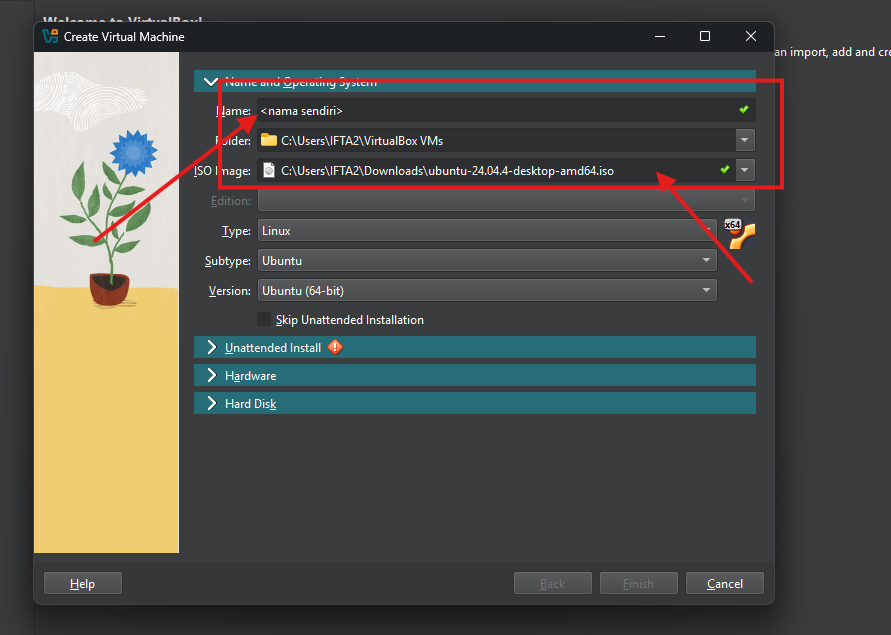
\includegraphics[width=0.75\textwidth]{Figure/02/gambar2.png}
            \caption{Tampilan Oracle VM VirtualBox saat memilih nama mesin virtual dan file ISO Ubuntu.}
            \label{fig:virtualbox-name-iso}
        \end{figure}

        \item Pada menu \textbf{Unattended Install}, isi \textbf{Username}, \textbf{Password}, dan \textbf{Hostname} (tanpa spasi), kemudian klik \textbf{Next}. 

        \begin{figure}[H]
            \centering
            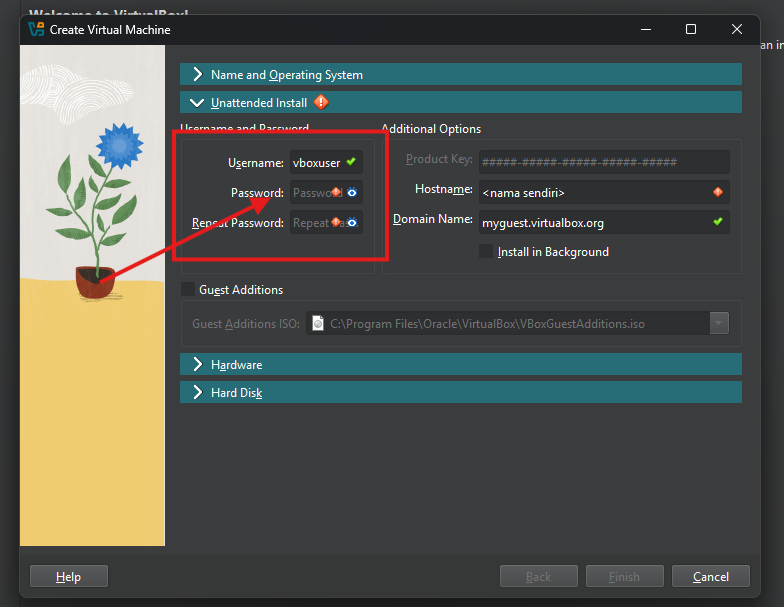
\includegraphics[width=0.75\textwidth]{Figure/02/gambar3.png}
            \caption{Tampilan Oracle VM VirtualBox pada tahap \textbf{Unattended Install}.}
            \label{fig:virtualbox-unattended-install}
        \end{figure}

        \item Pada menu \textbf{Hardware}, atur \textbf{Base Memory} minimal 4096 MB dan \textbf{Processor} minimal 2 core (sesuaikan dengan spesifikasi perangkat), lalu klik \textbf{Finish}. 

        \begin{figure}[H]
            \centering
            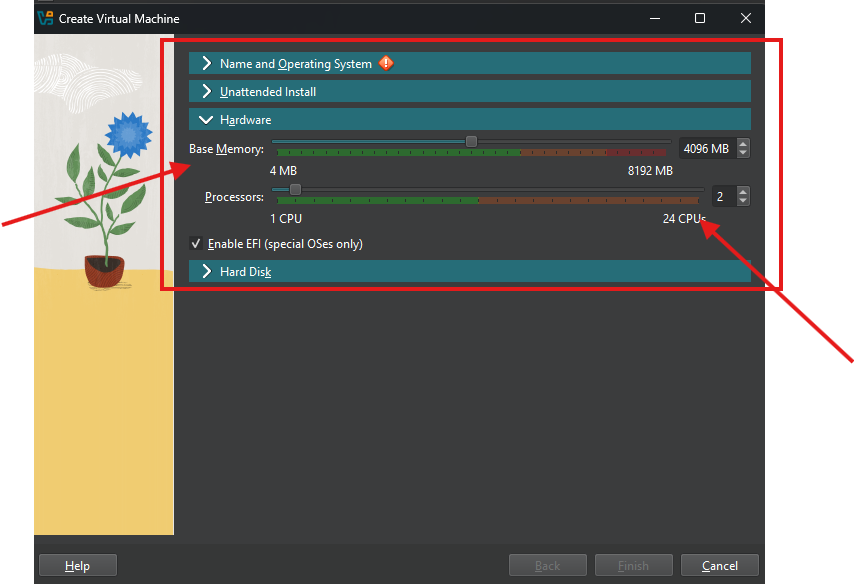
\includegraphics[width=0.75\textwidth]{Figure/02/gambar4.png}
            \caption{Tampilan pengaturan \textbf{Hardware} pada Oracle VM VirtualBox (Base Memory dan Processor).}
            \label{fig:virtualbox-hardware}
        \end{figure}

        \item Jalankan mesin virtual yang sudah dibuat, lalu pada tampilan awal instalasi pilih opsi \textbf{"Try or Install Ubuntu"}.

        \begin{figure}[H]
            \centering
            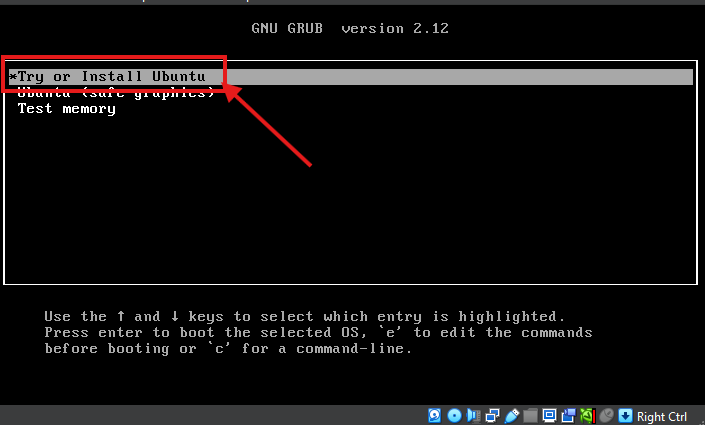
\includegraphics[width=0.75\textwidth]{Figure/02/gambar5.png}
            \caption{Tampilan awal instalasi Ubuntu saat memilih opsi \textbf{"Try or Install Ubuntu"}.}
            \label{fig:virtualbox-try-install}
        \end{figure}

        \item Lanjutkan proses instalasi sampai tahap \textit{copying files} selesai. Proses ini biasanya memerlukan waktu beberapa puluh menit, kemudian lakukan restart VM jika diminta. 
\end{enumerate}
\end{enumerate}

\newpage
\section{Latihan}

Pada bagian ini, setiap mahasiswa wajib mengerjakan tugas praktik mandiri sebagai berikut:
\begin{enumerate}
    \item Menginstal Ubuntu pada Oracle VM VirtualBox hingga sistem dapat berjalan dengan baik.
    \item Mendokumentasikan setiap langkah instalasi secara berurutan (wajib disertai bukti seperti tangkapan layar).
    \item Menyusun laporan praktikum sesuai template resmi pada GitHub IF ITERA:
    \url{https://github.com/informatika-itera/IF25-12007-Sistem-Operasi/tree/main/Hands-On}
\end{enumerate}

Laporan \textbf{wajib} disusun menggunakan \LaTeX.
